% \documentclass[letterpaper, 10 pt, conference]{ieeeconf}  % Comment this line out if you need a4paper
\documentclass[letterpaper, 10 pt, journal, twoside]{ieeetran}
% \IEEEoverridecommandlockouts                              % This command is only needed if 
                                                          % you want to use the \thanks command
% \overrideIEEEmargins                                      % Needed to meet printer requirements.
% \usepackage[top=60pt, left=48pt, right=48pt, bottom=43pt]{geometry}


% Bibliography
\usepackage{biblatex}
\addbibresource{references.bib}

% Math
\usepackage{physics}
\usepackage{siunitx}
\sisetup{output-exponent-marker=\ensuremath{\mathrm{e}}}
\usepackage{amsmath}
\usepackage{amsfonts}
\usepackage{amssymb}
\usepackage{gensymb}
\usepackage{tensor}

% Optimization and Algorithms
\usepackage{optidef}
\usepackage{algorithmicx}
\usepackage{algorithm,algpseudocode}

% Formatting
\usepackage{xcolor}
\usepackage{bm}  % for bold symbols 
\usepackage{booktabs}  % better tables
\usepackage{pifont}  % for x mark
\usepackage{graphicx}
\usepackage{hyperref}

% Plotting
\usepackage{pgfplots}
\pgfplotsset{compat=1.15,
	legend style={font=\footnotesize},
}
\usepackage{tikzscale}
\usepgfplotslibrary{fillbetween}
% \pgfplotsset{every axis plot post/.style={
%     very thick,
% }
% }

% Custom commands
\newcommand{\half}{\frac{1}{2}}
\newcommand{\R}{\mathbb{R}}
\newcommand{\Q}{\mathbb{S}^3}
\newcommand{\skewmat}[1]{[#1]^\times}

\newcommand{\rmap}{\varphi}
\newcommand{\invrmap}{\varphi^{-1}}

\DeclareMathOperator{\sign}{sign}

\newcommand{\dR}{\delta \mathcal{R}}
\newcommand{\rot}{ \mathcal{R} }
\newcommand{\dq}{\delta q}
\newcommand{\q}{\textbf{q}}
\newcommand{\eq}{_\text{eq}}
\newcommand{\traj}[2][N]{#2_{0:{#1}}}
\newcommand{\pass}{{\color{green} \checkmark}}
\newcommand{\fail}{{\color{red} \ding{55}}}
\newcommand{\inframe}[2]{{}^{#1}\!#2}
\newcommand{\toframe}[3]{\inframe{#1}{#3}^{#2}}

\newcommand{\todo}[1]{\textcolor{red}{TODO: #1}}
\newcommand{\added}[1]{\textcolor{black}{#1}}

% Header, Title, etc.
\markboth{IEEE Robotics and Automation Letters. Preprint Version. Accepted Dec, 2020}
{Jackson \MakeLowercase{et al.}: Planning with Attitude}

\title{\LARGE \bf
Planning with Attitude
}

% Make room for more info lines in the \author command 
\author{Brian E Jackson$^{1}$, Kevin Tracy$^{1}$, and Zachary Manchester$^{1}$%
\thanks{Manuscript received: October, 15, 2020; Revised January 2, 2021; Accepted January 4, 2021.}%Use only for final RAL version
\thanks{This paper was recommended for publication by Editor Nancy Amato upon evaluation of the Associate Editor and Reviewers' comments.
This work was supported by a NASA Early Career Faculty Award, NASA JPL, and NSF GFRP Grant No. DGE-1656518.} %Use only for final RAL version
\thanks{$^{1}$All authors are with the Robotics Institute, Carnegie Mellon University, Pittsburgh, PA, USA 
        {\tt\footnotesize brian.jackson@cmu.edu}}%
\thanks{Digital Object Identifier (DOI): see top of this page.}
}


\begin{document}
\maketitle

\begin{abstract}
Planning trajectories for floating-base robotic systems that experience large
attitude changes is challenging due to the nontrivial group structure of 3D
rotations. This paper introduces a powerful and accessible approach for
optimization-based planning on the space of rotations using only standard
linear algebra and vector calculus. We demonstrate the effectiveness of the
approach by adapting Newton's method to solve the canonical Wahba's problem,
and modify the trajectory optimization solver ALTRO to plan directly on the
space of unit quaternions, achieving superior convergence on problems
involving significant changes in attitude.
%\keywords{trajectory optimization, motion planning, control, quaternions}

\end{abstract}

\begin{IEEEkeywords}
    Motion and Path Planning, Optimization and Optimal Control, Computational Geometry, Underactuated Robots, Motion Control, 
\end{IEEEkeywords}

\section{INTRODUCTION}

    \IEEEPARstart{M}{any} robotic systems---including quadrotors, airplanes, satellites, autonomous
    underwater vehicles, and quadrupeds---can perform arbitrarily large three-dimensional
    translations and rotations as part of their normal operation. While representing
    translations is straightforward and intuitive, effectively representing the
    nontrivial group structure of 3D rotations has been a topic of study for many
    decades. Although we can intuitively deduce that rotations are three-dimensional, a
    globally non-singular three-parameter representation of the space of rotations does
    not exist \cite{stuelpnagel1964parametrization}. As a result, when parameterizing
    rotations, we must either a) choose a three-parameter representation and deal with
    singularities and discontinuities, or b) choose a higher-dimensional representation and deal with
    constraints between the parameters. While simply representing attitude is nontrivial,
    generating and tracking motion plans for floating-base systems is an even more
    challenging problem.

    Early work on control problems involving the rotation group dates back to the 1970s,
    with extensions of linear control theory to spheres \cite{Brockett1973} and $SO(3)$
    \cite{Baillieul1978}. Effective attitude tracking controllers have been developed for
    satellites \cite{wie1985quaternion}, quadrotors
    \cite{Fresk2013,Liu2015,lee2010geometric,
    Johnson2005,watterson2020control,mellinger2011minimum}, and a 3D inverted pendulum
    \cite{Chaturvedi2009} using various methods for calculating three-parameter attitude
    errors.

    More recently, these ideas have been extended to trajectory generation
    \cite{Zefran1998}, sample-based motion planning \cite{Zefran1999,Kuffner2004}, and
    optimal control. Approaches to optimal control with attitude states include
    analytical methods applied to satellites \cite{Spindler1998}, discrete mechanics
    \cite{Kobilarov2011,Kobilarov2014, Lee2008}, a combination of sampling-based planning
    and constrained trajectory optimization for satellite formations \cite{Garcia2005,
    Aoude2008}, projection operators \cite{Saccon2013}, or more general theory for
    optimization on manifolds \cites{watterson2018trajectory}. Nearly all of these
    methods rely heavily on principles from differential geometry and Lie group theory;
    however, despite these works, many recent papers in the robotics community continue
    to naively apply standard methods for motion planning and control with no regard for the
    group structure of rigid body motion.
    %\cite{Alothman2016,deCrousaz2015, Williams2017,Geisert2016}
    
    In this paper, we make a departure from previous approaches to geometric planning and
    control that rely heavily on ideas and notation from differential geometry, and
    instead use only basic mathematical tools from linear algebra and vector calculus
    that should be familiar to most roboticists. In Sec. \ref{sec:Quaternion_Calculus} we
    introduce an approach to quaternion differential calculus similar to
    \cite{Mandic2011,Xu2016}, but significantly simpler and more general, enabling
    straight-forward adaptation of existing algorithms to systems with quaternion states.
    For concreteness, we then apply our method to the canonical Wahba's
    problem~\cite{Wahba1965} in Sec. \ref{sec:Wahbas}, and demonstrate superior
    convergence to approaches that fail to properly account for the group structure. In
    Sec. \ref{sec:trajopt} we extend these ideas to the problem of trajectory
    optimization, and detail modifications to ALTRO, a state-of-the-art constrained
    trajectory optimization solver, and demonstrate performance gains on several
    benchmark problems. With the modifications presented in this paper, ALTRO explicitly 
    leverages both the structure of the trajectory optimization problem as well as the 
    group structure of 3D rotations, making it uniquely well-suited to solving challenging
    problems with near real-time performance.

    %To our knowledge, there does not currently exist a solver that is capable of leveraging the unique Markovian structure of the fixed-horizon trajectory optimization problem while correctly accounting for the group structure of 3D rotations. 
    In summary, our contributions include:

    \begin{itemize}
        \item A unified approach to quaternion differential calculus entirely based on
        standard linear algebra and vector calculus.
        \item Derivation of a Newton-based algorithm for nonlinear optimization directly
        on the space of unit quaternions.
        \item Implementation of a fast and efficient solver for trajectory optimization
        problems with attitude dynamics and nonlinear constraints that correctly accounts
        for the group structure of 3D rotations.
    \end{itemize}


\section{Background}

    We begin by defining some useful conventions and notation. 
    Attitude is defined as the rotation from the robot's body frame to the world frame.
    We also define gradients to be row vectors, that is, for 
        $f(x) : \R^n \to \R$, $\pdv{f}{x} \in \R^{1\times n}$.

    \subsection{Unit Quaternions} \label{sec:quaternions}
        We leverage the fact that quaternions are linear operators and that the space of
        quaternions $\mathbb{H}$ is isomorphic to $\R^4$ to explicitly
        represent---following the Hamilton convention---a quaternion $\q \in \mathbb{H}$
        as a standard vector $q \in \R^4 := [q_s \;\; q_v^T]^T$ where $q_s \in \R$ and
        $q_v \in \R^3$ are referred to as the scalar and vector parts of the quaternion,
        respectively. The space of unit quaternions, $\Q = \{q : \norm{q}_2 = 1\}$, is a 
        double-cover of the rotation group $SO(3)$, since $q$ and $-q$ represent the same 
        rotation \cite{markley2014fundamentals}.
        
        Quaternion multiplication is defined as
        \begin{equation} \label{eq:quat_mult}
            \q_2 \otimes \q_1 = L(q_2) q_1 = R(q_1) q_2
        \end{equation}
        where $L(q)$ and $R(q)$ are orthonormal matrices defined as
        \begin{align}
            L(q) &:= \begin{bmatrix} 
                q_s \;\; & -q_v^T \\ 
                q_v \;\; & q_s I + \skewmat{q_v} 
            \end{bmatrix} 
            \label{eq:Lmult} \\
            %= \begin{bmatrix} q & G(q) \end{bmatrix} \label{eq:Lmult} \\
            R(q) &:=\begin{bmatrix} 
                q_s \;\; & -q_v^T \\ 
                q_v \;\; & q_s I - \skewmat{q_v} 
            \end{bmatrix} \label{eq:Rmult},
        \end{align}
        and $\skewmat{x}$ is the skew-symmetric matrix operator
        \begin{equation}
            \skewmat{x} := \begin{bmatrix} 
                0 & -x_3 & x_2 \\ 
                x_3 & 0 & -x_1\\ 
                -x_2 & x_1 & 0 
            \end{bmatrix}.
        \end{equation}
        
        The inverse of a unit quaternion $\q^{-1}$, giving the opposite rotation, is equal 
        to its conjugate $\q^*$, which is simply the same quaternion with a negated vector 
        part:
        \begin{equation} \label{eq:T}
            \q^* = T q := \begin{bmatrix} 
                1 & \\ 
                & -I_3 
            \end{bmatrix} q.
        \end{equation}
        The following identities, which are easily derived from
        \eqref{eq:Lmult}--\eqref{eq:T}, are extremely useful:
        \begin{align}
            &L(Tq) = L(q)^T = L(q)^{-1} \\
            &R(Tq) = R(q)^T = R(q)^{-1} .
        \end{align}
        
        We will sometimes find it helpful to create a quaternion with zero scalar part from 
        a vector $r \in \R^3$. We denote this operation as,
        \begin{equation}
            \hat{r} = H r \equiv \begin{bmatrix} 0 \\ I_3 \end{bmatrix} r.
        \end{equation}
        Unit quaternions rotate a vector through the operation 
        $\hat{r}' = \q \otimes \hat{r} \otimes \q^*$. 
        This can be equivalently expressed using matrix multiplication as
        \begin{align} 
            r' &= H^T L(q) R(q)^T H r = A(q)r , \label{eq:quaternion_rotation}
        \end{align}
        where $A(q)$ is the rotation matrix in terms of the elements of the quaternion 
        \cite{kane1983spacecraftdynamics}.

    \subsection{Rigid Body Dynamics} \label{sec:rigidbody_dynamics}
        For clarity, we will restrict our attention to rigid bodies moving freely in 3D 
        space. That is, we consider systems with dynamics of the following form:
        \begin{equation} \label{eq:rigid_body_dynamics}
            x = \begin{bmatrix} r \\ q \\ v \\ \omega \end{bmatrix}, \quad 
            \dot{x} = \begin{bmatrix} 
                v \\ 
                \half \q \otimes \hat{\omega} = \half L(q) H \omega \\ 
                \frac{1}{m} \inframe{W}{F(x,u)} \\ 
                J^{-1}(\inframe{B}{\tau(x,u)} - \omega \times J \omega) 
            \end{bmatrix}
        \end{equation}
        where $x$ and $u$ are the state and control vectors, $r \in \R^3$ is the
        position, $\q \in \Q$ is the attitude, $v \in \R^3$ is the linear velocity, and
        $\omega \in \R^3$ is the angular velocity. $m \in \R$ is the mass, $J \in
        \R^{3\times3}$ is the inertia matrix, $\inframe{W}{F(x,u)} \in \R^3$ are the
        forces in the world frame, and $\inframe{B}{\tau(x,u)}$ are the moments in the
        body frame.

\section{Quaternion Differential Calculus} \label{sec:Quaternion_Calculus}
    We now present a simple but powerful method for taking derivatives of functions 
    involving quaternions based on the notation and linear algebraic operations outlined 
    in Sec. \ref{sec:quaternions}.
    
    \begin{figure}
        \centering
        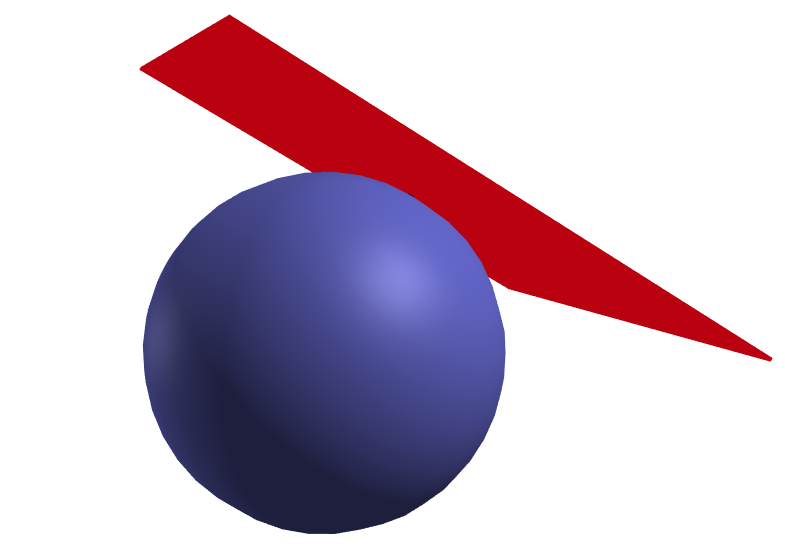
\includegraphics[height=5cm]{figures/tangent_plane.tikz}
        \caption{
            When linearizing about a point $q$ on an sphere $\mathbb{S}^{n-1}$ in 
            n-dimensional space, the tangent space $T$ is a plane living in $\R^{n-1}$, 
            illustrated here with $n=3$. Therefore, when linearizing about a unit 
            quaternion $q \in \Q$, the space of differential rotations lives in $\R^3$.
        }
        \label{fig:tangent_plane}
    \end{figure}
        
        Derivatives consider the effect an infinitesimal perturbation to the input has on
        an infinitesimal perturbation to the output. For vector spaces, the composition
        of the perturbation with the nominal value is simple addition and the
        infinitesimal perturbation lives in the same space as the original vector. For
        unit quaternions, however, neither of these are true; instead, they compose
        according to \eqref{eq:quat_mult}, and infinitesimal unit quaternions are (to
        first order) confined to a 3-dimensional plane tangent to $\Q$ (see Fig.
        \ref{fig:tangent_plane}).

        The fact that differential unit quaternions are three-dimensional should make
        intuitive sense: Rotations are inherently three-dimensional and differential
        rotations should live in the same space as angular velocities, i.e. $\R^3$.
        
        There are many possible three-parameter representations for small rotations in
        the literature. Many authors use the exponential map \cite{Baillieul1978,
        Zefran1998, Lee2008, Saccon2013, Sola2017, Fan2016, watterson2018trajectory},
        while others have used the Cayley map (also known as Rodrigues parameters)
        \cite{Kobilarov2011, Kobilarov2014}, Modified Rodrigues Parameters (MRPs)
        \cite{Terzakis2018}, or the vector part of the quaternion \cite{Fresk2013}.
        We choose Rodrigues parameters \cite{markley2014fundamentals} because they are
        computationally efficient and do not inherit the sign ambiguity associated with
        unit quaternions. The mapping between a vector of Rodrigues parameters $\phi \in
        \R^3$ and a unit quaternion $q$ is known as the Cayley map: \begin{equation}
        \label{eq:cayley}
            q = \varphi(\phi) = \frac{1}{\sqrt{1 + \norm{\phi}^2}} \begin{bmatrix} 1 \\ \phi \end{bmatrix}.
        \end{equation}
        We will also make use of the inverse Cayley map:
        \begin{equation}
            \phi = \varphi^{-1}(q) = \frac{q_v}{q_s}.
        \end{equation}

    \subsection{Jacobian of Vector-Valued Functions}
        When taking derivatives with respect to quaternions, we must take into account
        both the composition rule and the nonlinear mapping between the space of unit
        quaternions and our chosen three-parameter error representation.

        Let $\phi \in \R^3$ be a differential rotation applied to a function with
        quaternion inputs 
        $y = h(q): \Q \to \R^p$, such that
        \begin{equation} \label{eq:vector_function}
            y + \delta y = h(L(q) \varphi(\phi)) \approx h(q) +  \nabla h(q) \phi.
        \end{equation}
        \added{Note that we chose to represent $\phi$ in the body frame, consistent with the standard definition of angular velocity, and therefore it is applied to $q$ through right (rather than left) multiplication.} We can calculate the Jacobian $\nabla h(q) \in \R^{p \times 3}$ by
        differentiating \eqref{eq:vector_function} with respect to $\phi$, evaluated at
        $\phi = 0$:
        \begin{equation} \label{eq:quat_gradient}
            \nabla h(q) = \pdv{h}{q} L(q) H := \pdv{h}{q} G(q) 
                        = \pdv{h}{q} \begin{bmatrix} 
                            -q_v^T \\ 
                            q_s I_3 + \skewmat{q_v}
                        \end{bmatrix}
        \end{equation}
        where $G(q) \in \R^{4 \times 3}$ is the \textit{attitude Jacobian}, which
        essentially becomes a ``conversion factor'' allowing us to apply results from
        standard vector calculus to the space of unit quaternions. This form is
        particularly useful in practice since $\pdv*{h}{q} \in \R^{p \times 4}$ can be
        obtained using finite differences or automatic differentiation.
        As an aside, although we have used Rodrigues parameters, $G(q)$ is actually the
        same (up to a constant scalar factor) for any choice of three-parameter attitude
        representation.

    \subsection{Hessian of Scalar-Valued Functions}
	    If the output of $h$ is a scalar ($p = 1$), then we can find its Hessian by
	    taking the Jacobian of \eqref{eq:quat_gradient} with respect to $\phi$ using the
        product rule, again evaluated at $\phi = 0$:

	    \begin{equation} \label{eq:quat_hessian}
            \nabla^2 h(q) = G(q)^T \pdv[2]{h}{q} G(q) + I_3 \pdv{h}{q}q,
	    \end{equation}
	    where the second term comes from the second derivative of $\varphi(\phi)$.
	    Similar to $G(q)$, this expression is the same (up to a constant scalar factor) for any
        choice of three-parameter attitude representation.
        
    \subsection{Jacobian of Quaternion-Valued Functions}
        We now consider the case of a function that maps unit quaternions to unit
        quaternions, $q' = f(q) : \Q \to \Q$. 
        % \todo{Let's make sure we're bing consistent with our usage of $\Q$ vs. $\mathbb{H}$.} 
        Here we must also consider the non-trivial
        effect of a differential rotation applied to the output, i.e.:
        \begin{equation} \label{eq:dqoutput}
            L(q') \varphi(\phi') = f(L(q)\varphi(\phi)) .
        \end{equation}
        Solving \eqref{eq:dqoutput} for $\phi'$ we find,
        \begin{equation} \label{eq:phiprime}
            \phi' = \varphi^{-1} \left( L(q')^T f(L(q)\varphi(\phi)) \right) \approx \nabla f(q) \, \phi.
        \end{equation}
        Finally, the desired Jacobian is obtained by taking the derivative of
        \eqref{eq:phiprime} with respect to $\phi$:
        \begin{equation} \label{eq:quat_jacobian}
            \nabla f(q) = H^T L(q')^T \pdv{f}{q} L(q) H = G(q')^T \pdv{f}{q} G(q).
        \end{equation}
        %The leading $G(q')^T$ comes from the fact that as $\phi' \to 0$, $L(q') f(q) \to
        %I_q$, where $I_q$ is the quaternion identity.
        Once again, \eqref{eq:quat_jacobian} holds (up to a constant) for any
        three-parameter attitude representation.
        
        %Differentiating through the inverse map, evaluated at the quaternion identity, we find that $\pdv*{\varphi^{-1}}{q}\to H^T$ for any three-parameter attitude representation.


\section{Modifying Newton's Method} \label{sec:Wahbas}

% \todo{I would re-work this section to only talk about the details of doing it the ``correct'' way (i.e. consistent with the previous section). Then just call the standard version a ``naive Newton method in which the quaternion is re-normalized at each step'' and don't bother writing any of the mathematical details for that version. I think it will get confusing if you mix derivative types/notation.}

    Newton's method uses derivative information about a function to iteratively
    approximate its roots. For unconstrained systems, this method is highly effective,
    and can exhibit quadratic convergence rates. For constrained systems, the updates 
    can be projected back onto the feasible set at each iteration, but without the same
    convergence guarantees.
    %For the constraints on $SO(3)$, Newton's method struggles to
    %converge past a certain threshold due to this projection.
    
    In this section, we will leverage the quaternion calculus results introduced in the previous section to modify Newton's method so that it implicitly accounts for the quaternion unit-norm constraint. Unlike the projection approach, this modified form of Newton's method retains the fast convergence rates associated with the unconstrained method. We will demonstrate this behavior on Wahba's Problem, a least-squares attitude estimation problem~\cite{Wahba1965, markley2014fundamentals}.
    

    \subsection{Methodology}
% \todo{Let's keep our notation and language consistent for body vs. inertial frames. I propose ``body'' (B) and ``inertial'' or ``world'' (W), which is the standard in robotics.}
    Given a set of known vectors in the world frame, $\inframe{W}{w_i}$, and measurements of these vectors in the body frame, $\inframe{B}{v_i}$, we seek the
    rotation from the body to the world frame $\toframe{W}{B}{A(q)}$ that solves the following optimization problem,
    \begin{mini*}
        {q}{ W(q) }{}{}
        \addConstraint { q\in \Q,}
    \end{mini*}
    where Wahba's loss function $W(q)$ is,
    \begin{equation} \label{eq:wahba_loss}
        W(q) = \sum_i \norm{\inframe{W}{w_i} - A(q) \,\, \inframe{B}{v_i} }_2^2 
           = \norm{r(q)}_2^2 ,
    \end{equation} 
    and $r(q)$ is the residual vector.


    The Jacobian of $r(q)$ can be found using \eqref{eq:quat_gradient}:
    \begin{align} \label{eq:newton_foc}
            \nabla r(q) &= \pdv{r}{q} G(q) \\
              &= -2 H^T R(q)^T \left( \sum_i R({}^B \hat{v}_i) \right) G(q) .
    \end{align} 
    Given a guess solution, $q_k$, The standard Gauss-Newton method can then be used to compute a three-parameter update, $\phi_k$ via the Moore-Penrose psuedoinverse:

    \begin{equation}
    	\phi_k = ({\nabla r}^T {\nabla r})^{-1} {\nabla r}^T r(q_k).
    \end{equation}
	The update is then applied using the composition for the group:
	\begin{equation}
		\q_{k+1} = \q_k \otimes \varphi(\phi_k).
	\end{equation}
	This ``multiplicative'' Gauss-Newton method is summarized in Algorithm \ref{alg:mgn}.

    \begin{algorithm} 
    	\begin{algorithmic}[1]
    		\caption{Multiplicative Gauss-Newton Method}\label{alg:mgn}
    		\State $k = 0$
    		\While{$\norm{\phi} > $ tolerance}
    		    \State ${\nabla r} = \pdv{r(q_k)}{q} G(q_k)$ 
    		    	\Comment{Compute Jacobian}
    		    \State $ \phi = -({\nabla r}^T {\nabla r})^{-1} {\nabla r}^T r(q_k)$ \Comment{Compute update step}
    		    \State $q_{k+1} = L(q_k) \varphi(\phi)$ \Comment{Apply update step}
    		    \State $k = k + 1$
    		\EndWhile
    	\end{algorithmic}
    \end{algorithm}



    \subsection{Results} Figure \ref{fig:wahba_convergence} compares the
    multiplicative Gauss-Newton method with a na\"ive Newton's method in
    which the quaternion is simply projected back onto the unit sphere at
    every iteration. The na\"ive method makes progress initially, but quickly
    stalls. By correctly handling the group structure of unit quaternions,
    the multiplicative method is able to maintain the fast convergence rates
    typical of Newton's method. \added{By comparing our method with the
    global solution obtained from a singular-value decomposition
    \cite{markley1999estimate}, we see that our method recovers the globally
    optimal solution within a small number of iterations.} 
    
    \begin{figure}
        \centering
        \includegraphics[width=\columnwidth, height=5cm]{figures/wahba_convergence.tikz}
        \caption{Convergence comparison for Wahba's problem. \added{The error
        is the angle between the current solution and the globally optimal
        solution computed using a singular-value decomposition.
        The thick line is the average result of 100 trials with randomized
        orientations and measurements. The thin lines are the maximum and
        minimum over all 100 trials.} By modfying Newton's method with the
        methods of section \ref{sec:Quaternion_Calculus}, quadratic
        convergence rates are achieved, while a na\"ive approach stalls after
        only a few iterations.}
        \label{fig:wahba_convergence}
    \end{figure}

\section{Trajectory Optimization \added{for Rigid Bodies}} \label{sec:trajopt}
    Here we outline the modifications to the ALTRO solver \cite{howell2019altro} to
    solve trajectory optimization problems for rigid bodies, which extends easily to
    arbitrary systems whose state is in $\R^n \times \added{\Q}$. %ALTRO is an efficient solver for constrained nonlinear optimization problems that uses iterative LQR (iLQR) with an augmented Lagrangian framework.
    We consider trajectory optimization problems of the form,
    \begin{mini}[2]
        {x_{1:N},u_{1:N-1}}{\ell_f(x_N) + \sum_{k=1}^{N-1} \ell_k(x_k,u_k) }{}{}
        \addConstraint{x_{k+1} = f(x_k,u_k)}
        \addConstraint{g_k(x_k,u_k)}{\leq 0}
        \addConstraint{h_k(x_k,u_k)}{=0}
        \label{discrete_trajopt},
    \end{mini}
    where $x$ and $u$ are the state and control vectors as described in Sec. \ref{sec:rigidbody_dynamics},
    $f$ are the dynamics as defined in \eqref{eq:rigid_body_dynamics}, $\ell_k$ is a general
    nonlinear cost function at a single time step,
    $N$ is the number of time steps, and $g_k$, $h_k$ are general nonlinear inequality and 
    equality constraints.

    ALTRO combines techniques from both differential dynamic programming (DDP) and direct transcription methods to achieve high performance on challenging constrained nonlinear trajectory optimization problems. Like most methods for nonlinear optimization, ALTRO iteratively approximates the
    nonlinear functions $f, \ell, g,$ and $h$ with their first or second-order Taylor
    series expansions. Leveraging the methods from Sec: \ref{sec:Quaternion_Calculus}, we
    adapt the algorithm to optimize directly on the error state $\delta x \in \R^{12}$:
    \begin{equation} \label{eq:state_error}
    	\delta x_k = \begin{bmatrix} 
            r_k - \bar{r}_k \\ \varphi^{-1}(\bar{\q}_k^{-1} \otimes \q_k) \\ v_k - \bar{v}_k \\ \omega_k - \bar{\omega}_k 
        \end{bmatrix}.
    \end{equation}

    We begin by linearizing the dynamics about the reference state and input trajectories, $\bar{x}$ and $\bar{u}$, using
    \eqref{eq:quat_jacobian}. The linearized error dynamics become,
    \begin{equation} \label{eq:linearized_dynamics}
        \delta x_{k+1} = A_k \delta x_k + B_k \delta u_k ,
    \end{equation}
    where \begin{equation}
        \begin{aligned}
            A_k = E(\bar{x}_{k+1})^T \pdv{f}{x}|_{\bar{x}_k,\bar{u}_k} E(\bar{x}_k), \\
            B_k = E(\bar{x}_{k+1})^T \pdv{f}{u}|_{\bar{x}_k,\bar{u}_k},
        \end{aligned}
    \end{equation}
    and $E(x_k) \in \R^{12 \times 13}$ is the error-state Jacobian:
    \begin{equation} \label{eq:state_error_jacobian}
        E(x) = \begin{bmatrix}
            I_3 & & & \\
            & G(q) & & \\
            & & I_3 & \\
            & & & I_3 \\
        \end{bmatrix}\!.
    \end{equation}
    By applying \eqref{eq:quat_gradient} and \eqref{eq:quat_hessian} to the nonlinear
    cost functions $\ell$ and \eqref{eq:quat_jacobian} to the nonlinear constraint
    functions $g_k$ and $h_k$, we can calculate the second-order expansion of the cost 
    function:
    \begin{multline}
        \delta \ell(x,u) \approx  \half \delta x^T \ell_{xx} \delta x
            + \half \delta u^T \ell_{uu} \delta u + \delta_u^T \ell_{ux} \delta u \\
            + \ell_x^T \delta x^T + \ell_u^T \delta u.
    \end{multline}
    % \todo{I think you can safely leave out any references to the augmented Lagrangian,
    % etc. and just talk about the cost function.}
    % \begin{equation}
    %     \mathcal{L}_A = \mathcal{L}_N(x_N,\lambda_N,\mu_N) + 
    %         \sum_{k=0}^{N-1} \mathcal{L}_k(x_k,u_k,\lambda_k,\mu_k)
    % \end{equation}
    % where
    % \begin{equation}
    %     \mathcal{L}_k(x,u,\lambda,\mu) = \ell(x,u) + 
    %         (\lambda + \half I_\mu c(x,u))^T c(x,u),
    % \end{equation}
    % with $c(x,u)$ being the concatenation of the constraints $f,g$, and $h$ at a given time step,
    % and $I_\mu$ the penalty matrix.
	
	With these results, we can apply standard Newton and quasi-Newton techniques along the lines of Section \ref{sec:Wahbas}. We can also calculate a second-order expansion of the ``action-value function'' $Q(x,u)$ needed in DDP and LQR-based methods,
    \begin{align}
        Q_{xx} &= \ell_{xx} + A_{k}^T P_{k+1} A_{k} \label{Qxx_exp}\\
        Q_{uu} &= \ell_{uu} + B_{k}^T P_{k+1} B_{k} \label{Quu_exp}\\
        Q_{ux} &= \ell_{ux} + B_{k}^T P_{k+1} A_{k} \label{Qux_exp}\\
        Q_x &= \ell_x  + A_{k}^T p_{k+1} \label{Qx_exp}\\
        Q_u &= \ell_u + B_{k}^T p_{k+1} \label{Qu_exp},
    \end{align}
    from which we can calculate the quadratic expansion of the cost-to-go 
    $P_k \in \R^{12 \times 12}$, $p_k \in \R^{12}$, and optimal linear feedback gains 
    $K_k \in \R^{m \times 12}$ and feed-forward corrections $d_k \in \R^m$ by starting at the terminal state and
    performing a backward Riccati recursion as usual~\cite{li2004iterative,howell2019altro}.
    
    During the ``forward rollout'' of these methods, the dynamics are simulated forward in time using updated control inputs: 
    \begin{equation} \label{eq:mlqr_control}
        u_k = \bar{u}_k - d_k - K_k \delta x_k.
    \end{equation}
    where $\bar{u}_k$ is the control value from the previous iteration, and $\delta x$ is
    computed using \eqref{eq:state_error}. %, with $x_k$ being the current state estimate and $\bar{x}_k$ the state from the previous iteration. 
    For more details on the ALTRO algorithm, we refer the reader to~\cite{howell2019altro}.

    \subsection{Quaternion Cost Functions} \label{sec:cost_functions}
        In addition to the straight-forward modifications to the ALTRO algorithm itself, some care must be taken in designing cost functions that are well-suited to unit quaternions. We
        frequently minimize costs that penalize distance from a goal state, e.g. $\half
        (x-x_g)^T Q (x-x_g)$; however, na\"ive substraction of unit quaternions does not respect their group structure, and often results in undesired behavior. Instead, we have found the following cost function, which penalizes the geodesic
        distance between two unit quaternions \cite{Kuffner2004}, to work well in practice:
        \begin{equation} \label{eq:quat_geodesic}
            J_\text{geo} = (1-\abs{q_g^T q}) .
        \end{equation}
        Its gradient and Hessian are,
        \begin{align}
            \nabla J_\text{geo} &= \sign(q_d^T q) q_g^T G(q) \\
            \nabla^2 J_\text{geo} &= \sign(q_d^T q) I_3 q_g^T q ,
        \end{align}
        where $\sign$ denotes the signum function. \added{This cost function is particularly
        useful for rotations since it eliminates the ambiguity arising from the quaternion 
        double-cover of $SO(3)$.}
        
        % \subsubsection{Error Quadratic} \label{sec:error_quadratic}
        %     Rather than simple subtraction, we can use a quadratic function on the
        %     three-parameter error state \eqref{eq:state_error}:
        %     \begin{equation} \label{eq:error_quadratic}
        %         J_\text{err} = \half \phi^T Q \phi 
        %         = \half \left(\varphi^{-1}(\delta q)\right)^T Q 
        %                 \left(\varphi^{-1}(\delta q)\right).
        %     \end{equation}
        %     where $\delta q = L(q_g)^T q$, and $\phi = \varphi{\delta q}$. The gradient
        %     and Hessian of \eqref{eq:error_quadratic} are
        %     \begin{equation}
        %         \nabla J_\text{err }= \phi^T Q  D(\delta q)  G(\delta q)
        %     \end{equation}
        %     \begin{multline}
        %         \nabla^2 J_\text{err} = 
        %             G(\delta q)^T \! \left(
        %             D(\delta q)^T Q D(\delta q) + \nabla D \right) G(\delta q)  \\
        %             + I_3 (\phi^T Q  D(\delta q)) \delta q %\\
        %     \end{multline}
        %     where, for the Cayley map,
        %     \begin{equation}
        %         D(q) = \pdv{\varphi^{-1}}{q} = -\frac{1}{q_s^2}\begin{bmatrix}
        %             q_v \;\; & -\frac{1}{q_s} I_3
        %         \end{bmatrix}
        %     \end{equation}
        %     \begin{equation}
        %         \nabla D = \pdv{q}(D(q)^T Q \phi) 
        %         = -\frac{1}{q_s^2} \begin{bmatrix} 
        %             -2 \frac{q_v}{q_s}^T Q \phi & \phi^T Q \\
        %                            Q \phi & 0 \\
        %         \end{bmatrix}.
        %     \end{equation}

        % \subsubsection{Geodesic Distance} \label{sec:geodesic}

% \todo{If the geodesic distance works better on all the examples, I vote for leaving out the error quadratic stuff.}

\section{Experiments} \label{sec:experiments}
    In this section we present several trajectory optimization problems for systems that
    undergo large changes in attitude: an airplane barrel roll, a quadrotor flip, and a
    satellite with flexible solar panels that must slew to a new orientation while
    avoiding a keep-out zone.    
    All problems are run using ALTRO, first without any of the modifications presented in
    the current paper, analagous to the na\"ive Newton's method in section \ref{sec:Wahbas}
    and labeled ``naive'', and then using the modifications listed in Sec.
    \ref{sec:trajopt} and the geodesic cost function described in Sec.
    \ref{sec:cost_functions}, labeled ``modified''. All cost functions are of the
    following form:
    \begin{align}
        \ell_\text{naive}(x, u, \bar{x}, Q, R) &= \half (x - \bar{x})^T Q (x - \bar{x}) + \half u^T R u \\
        \ell_\text{modified}(x, u, \bar{x}, Q, R) 
            &= \ell_\text{naive}(x, u, \bar{x}, \bar{Q}, R) + w (1 \pm \bar{q}^T q)
    \end{align}
    where $\bar{x}$ is the reference state and $\bar{Q} = \text{diag}(Q_r, \vec{0}_4,
    Q_v, Q_\omega)$, with $Q_r,Q_v,Q_\omega$ being the weights of $Q$ for position, and
    linear and angular velocity, respectively.
    
    Timing results are summarized in Table \ref{tab:timing_results}. All experiments are 
    solved to a constraint satisfaction tolerance of $10^{-5}$ and discretized with a 4th 
    order Runge-Kutta integrator. The results were run on a laptop computer with a 2.8 GHz 
    i7-1165G7 processor with 16 GB of RAM. Code for all experiments is available on
    \href{https://github.com/RoboticExplorationLab/PlanningWithAttitude}
    {GitHub\footnote{\url{https://github.com/RoboticExplorationLab/PlanningWithAttitude}}}.

    \begin{table}
        \centering
        \caption{Trajectory Optimization Timing Results (naive/modified)}
        \begin{tabular}{lll}
\toprule 
Problem & Iterations & time (ms) \\
\midrule 
barrellroll & 47 / 36 & 94.54 / 78.65 \\
quadflip & 58 / 28 & 457.58 / 217.69 \\
satellite & 35 / 35 & 446.52 / 517.47 \\
\bottomrule 
\end{tabular}

        \label{tab:timing_results}
    \end{table}
        
    \subsection{Airplane Barrel Roll}
% \todo{Reference \eqref{eq:rigid_body_dynamics} and then say that the forces and torques due to lift and drag are fit from wind tunnel data. Also, cite that paper.}

        A 180 degree barrel roll trajectory for a fixed-wing airplane was
        optimized. The airplane's dynamics model consists of the a simple
        rigid body as defined in Section \ref{sec:rigidbody_dynamics} with
        forces and torques due to lift and drag fit from wind tunnel data
        \cite{manchester2016udp}. The airplane was tasked to do a barrel roll
        by constraining the terminal state to upside-down (see Fig.
        \ref{fig:barrellroll}). To mitigate issues with integration error and
        drift in the magnitude of the quaternion, the following constraint
        function was used to enforce a terminal orientation of $\bar{q}$:
        \begin{equation}
            \frac{q_v}{\norm{q}} - \bar{q}_v
                \sign\left(\bar{q}^T \frac{q }{ \norm{q}}\right) = 0
        \end{equation}

        The solver was initialized with level flight trim
        conditions. The convergence of the different versions of ALTRO is compared in
        Fig. \ref{fig:c_max_convergence}. As expected, the modified version achieves
        better convergence and faster solve times compared to the na\"ive version since
        the expansions being provided to the algorithm more accurately capture the
        relationship between the attitude state and the goal and constraints. For this 
        relatively simple problem, we gained a modest 31\% improvement in runtime, despite
        the additional matrix multiplications when calculating the cost and constraint
        expansions.

        \begin{figure}[t]
            \centering
            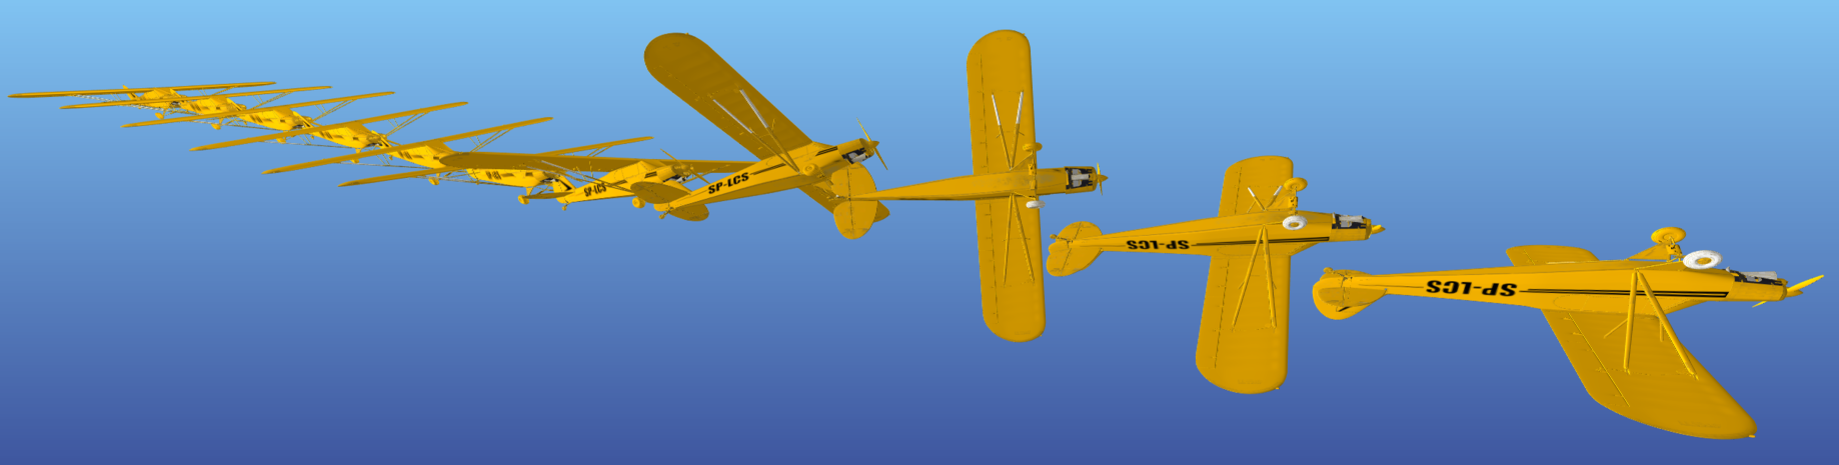
\includegraphics[width=\columnwidth]{figures/barrellroll.png}
            \caption{Barrel roll trajectory computed by ALTRO using a terminal cost to encourage an upside-down attitude.}
            \label{fig:barrellroll}
        \end{figure}

        \begin{figure}[t]
            \centering
            \includegraphics[height=4cm,width=\columnwidth]{figures/c_max_convergence.tikz}
            \caption{Constraint satisfaction as a function of iteration when solving the barrel roll problem using ALTRO both with and without the modifications for optimizing unit quaternions.}
            \label{fig:c_max_convergence}
        \end{figure}

    \subsection{Quadrotor Flip}
        A 360 degree flip trajectory for a quadrotor was optimized with dynamics adapted
        from \cite{mellinger2012trajectory}. To encourage the flip, we specified a 
        ``waypoint'' cost function of the following form:
        \begin{multline}
                  \sum_{k \in \mathcal{N}} \ell(x_k, u_k, \hat{x}, \hat{Q}, R) 
                + \sum_{k \in \mathcal{W}} \ell(x_k, u_k, \bar{x}_k, Q_w, R) 
        \end{multline}
        where $\hat{x}$, $\hat{Q}$ are the nominal state and state weight matrix, $Q_w$ is 
        the weight matrix for the waypoints, and
        $\mathcal{W} = \{20,45,51,55,75,101\}$, $\mathcal{N} = \{1:101\} \setminus
        \mathcal{W}$.
        Four intermediary ``waypoints'' were used to encourage the quadrotor
        to reach angles of \ang{90}, \ang{180}, \ang{270}, and \ang{360}
        around an approximately circular arc. The last waypoint was used to
        encourage the quadrotor to move towards the final goal, and the first
        kept it above the floor before starting the loop. The solver was
        provided a dynamically infeasible initial trajectory that linearly
        interpolates between the initial and final states, rotating the
        quadrotor around the x-axis a full \ang{360}.

	    Figure \ref{fig:quad_flip} shows snapshots of the trajectory as
	    generated using ALTRO. \added{To compare the convergence properties of the
	    two methods, the optimal state and control trajectories were
	    perturbed with random Gaussian white noise with a mean of 1 for
	    position, linear velocity, and angular velocity, 0.1 for the
        controls, and 145 degrees for the orientation (about a random axis). 
        As shown in Fig. \ref{fig:flip_success}, the modified method converges
        more reliably than the na\"ive method.}
	    It is also worth noting that this problem could not be solved using
	    any three-parameter attitude representation, since it passes through
	    the singularities at $90\degree, 180\degree$, and $360\degree$
	    associated with Euler angles, Rodrigues parameters, and Modified
	    Rodrigues Parameters, respectively.

        \begin{figure}[t]
            \centering
            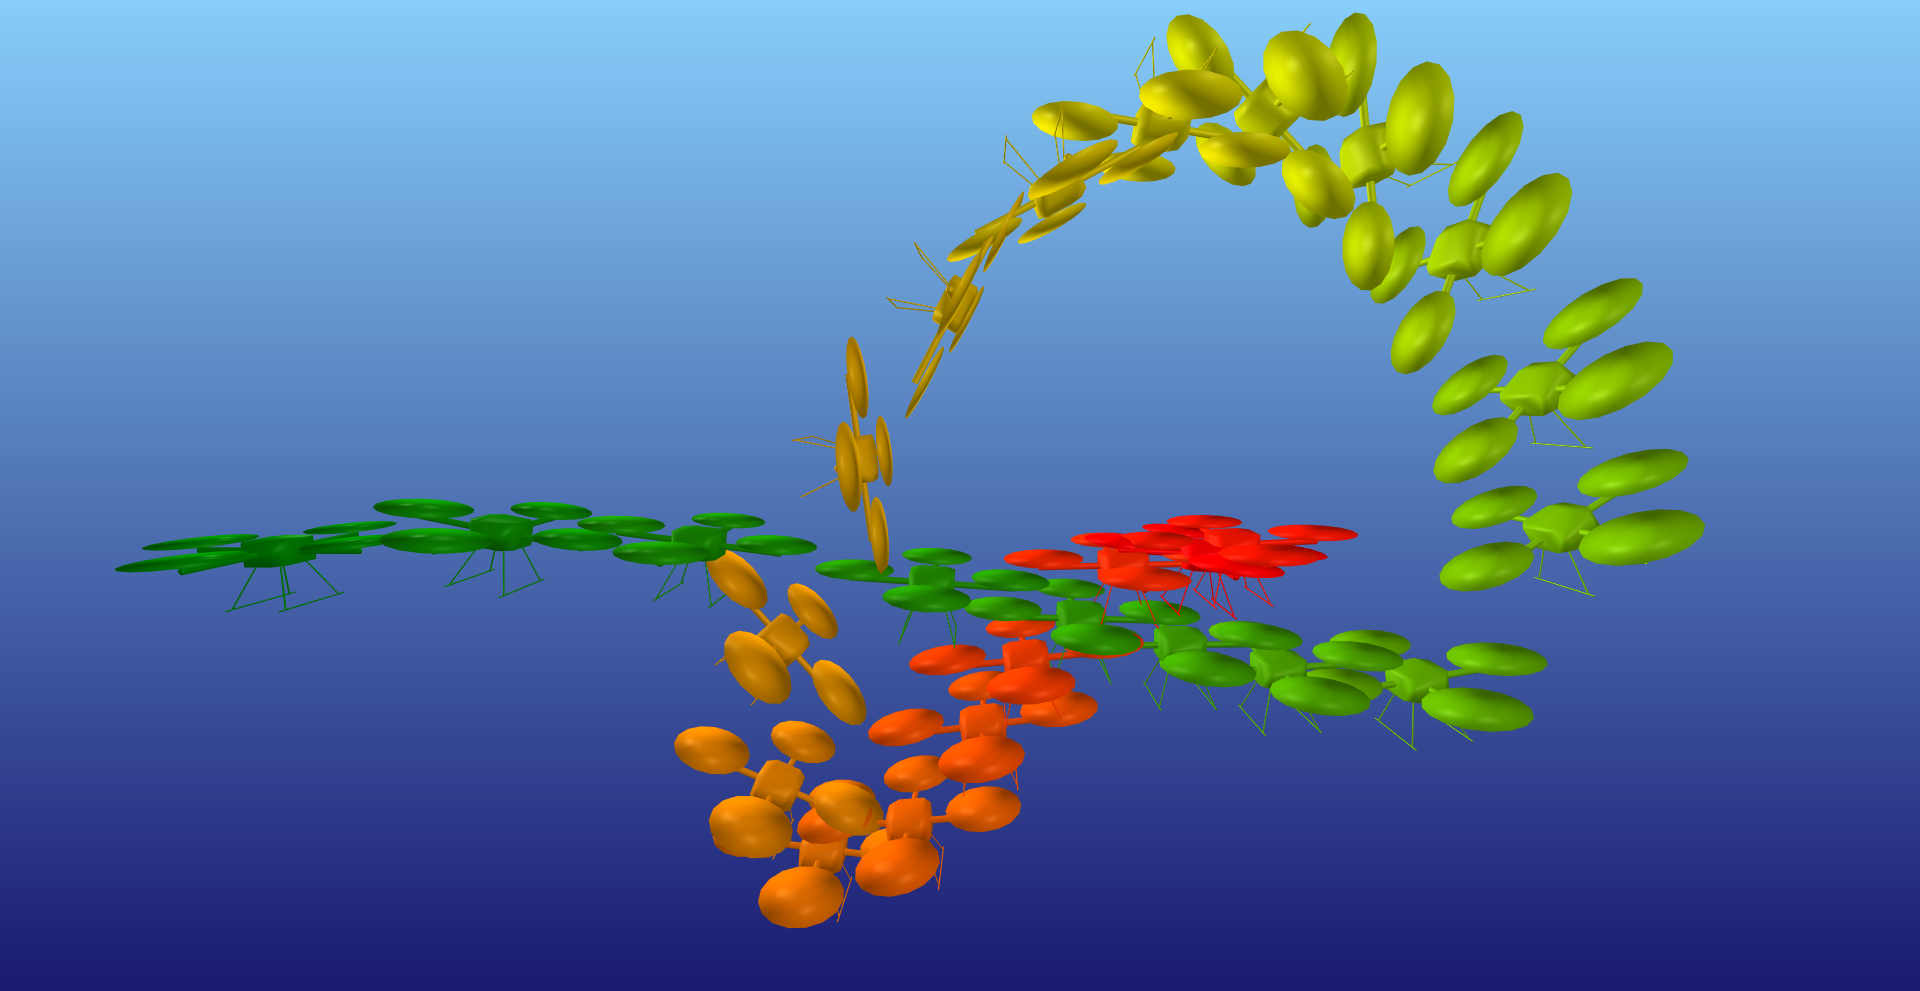
\includegraphics[width=\columnwidth]{figures/quadflip.png}
            \caption{Snapshots of the quadrotor flip trajectory. The
                gree-colored quadrotors represent the state near t=0 s and the
                red-colored quadrotors represent the state near t=5.0 s
            }
            \label{fig:quad_flip}
        \end{figure}

        \begin{figure}
            \centering    
            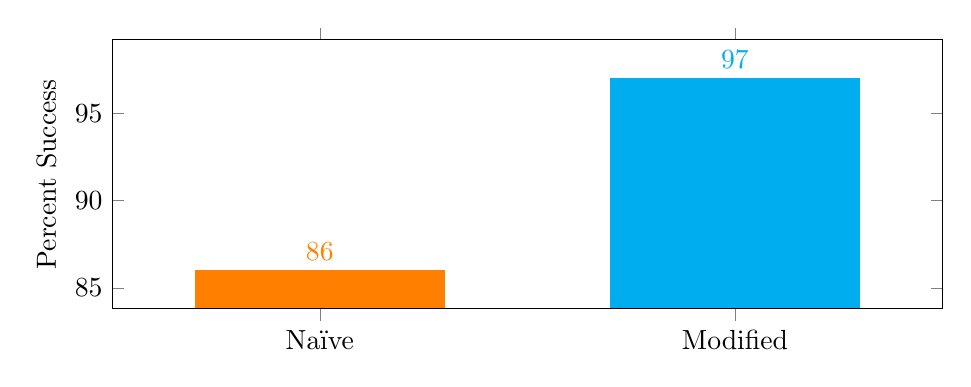
\begin{tikzpicture}
                \begin{axis}[
                    ybar,
                    width=\columnwidth, 
                    height=5cm, 
                    enlarge x limits=0.5,
                    enlarge y limits=0.2,
                    ylabel={Percent Success},
                    xtick={1,2},
                    xticklabels={Na\"ive, Modified},
                    bar width=0.6,
                    nodes near coords,
                    bar shift=0pt,
                    axis on top
                ]
                \addplot [orange, fill] coordinates {(1,86)};
                \addplot [cyan, fill]   coordinates {(2,97)};
                \end{axis}
            \end{tikzpicture}
            \caption{Convergence comparison for quadrotor flip. Percent of 100 trials 
            that successfully converged, where each trial is initialized with locally-optimal
            trajectories perturbed with significant Gaussian white noise.}
            \label{fig:flip_success}
        \end{figure}


    \subsection{Satellite Attitude Keep-Out}
        % \todo{Let's add a little more detail here: How about saying the dynamics are \eqref{eq:rigid_body_dynamics} plus a few extra states to capture the bending modes. Also, let's just call the start tracker a camera or sensor.}
        A spacecraft with flexible appendages was tasked to perform a 150 degree slew maneuver while
        ensuring that a body-mounted camera did not point within 40 degrees of a  ``keep-out zone'' around the sun vector. The spacecraft dynamics are presented in detail in~\cite{Tracy2020}, and are based
        on equation \eqref{eq:rigid_body_dynamics} with the addition of six states to account for three flexible modes. Control torques are generated by four reaction wheels.  A quadratic cost function penalizes error from the desired final attitude as well as displacement of the flexible modes. 
        % \todo{Kevin: add some info on cost function, initial guess (if any), etc.}
        We enforce the camera keep-out zone with the following constraint,
        \begin{equation}
            \left(\inframe{W}{r_{sun}}\right)^T 
            \left(\toframe{W}{B}{A(q)} \, \inframe{B}{r_{cam}} \right) \leq \cos(40 ^\circ) ,
        \end{equation}
        where $^Br_{cam}$ is the camera line-of-sight unit vector in the body frame and $^Wr_{sun}$ is the unit vector pointing to the sun in the world frame. The attitudes that satisfy this constraint comprise a non-convex set, with the constraint itself being nonlinear in $q$.
        \begin{figure}[ht]
            \centering
            \includegraphics{figures/kevins_plots/attitude_slew_plot.tikz}
            \caption{Visualization of the flexible spacecraft slew with a keep-out zone. Attitude is parameterized with a Rodrigues parameter to visualize the trajectory in three dimensions. The constraint surface represents attitudes where the camera line-of-sight is within 40$^\circ$ of the sun. The unconstrained solution violates this constraint, while the constrained solution is able to avoid the keep out zone.}
            \label{fig:keepout}
        \end{figure}
        
        ALTRO is able to converge to a locally optimal trajectory for this problem without an initial guess (all controls were initialized to zero). The resulting attitude trajectory is depicted in Fig. \ref{fig:keepout}. Without enforcing the camera constraint, the trajectory passes through the keep-out zone. As noted in Table \ref{tab:timing_results}, the quaternion modifications did not result in a significant improvement over the naive implementation of ALTRO for this problem, indicating that the computational benefits are problem dependent. We hypothesize that the more dynamic behaviors in the other examples benefit more from the quaternion modifications than the relatively slow-moving spacecraft.
    

\section{Conclusions} \label{sec:conclusion}
    We have presented a general, unified method for optimization-based planning and control for rigid-body
    systems with arbitrary attitude using standard linear algebra and vector calculus.
    The application of this methodology is straightforward and
    yields substantial improvements in the convergence of Newton and DDP-based methods, while also offering improvements for nonlinear constrained
    trajectory optimization for floating-base systems.
    
    Many state-of-the-art trajectory optimization methods, including direct collocation and sequential convex programming, rely on general-purpose optimization solvers whose internal numerical methods are not exposed to the user. Therefore, these methods are unable to exploit the full structure of both the trajectory optimization problem and the rotation group at a low level. In contrast, we are able to implement deep, native support for quaternions into the ALTRO solver, making it possible to solve more challenging problems with higher performance than other algorithms.

    In future work, we plan to apply ALTRO to real-time model-predictive control problems for aerial vehicles like quadrotors and airships that experience large attitude changes. The methods we have presented can also be leveraged to adapt other classes of gradient or Newton-based algorithms to exploit the structure of 3D rotations. Future directions beyond trajectory optimization may include simulation and planning methods that leverage maximal-coordinate formulations of multi-body dynamics~\cite{brudigam2020linear}, system-identification for complex multi-body systems and fixed-wing aircraft in post-stall conditions, and state estimation for spacecraft with sparse measurements. 

\section*{Acknowledgements}
This work was supported by a NASA Early Career Faculty Award (Grant Number 80NSSC18K1503).
This research was carried out in part at the Jet Propulsion Laboratory, California Institute of Technology, under a contract with the National Aeronautics and Space Administration and funded through JPL’s Strategic University Research Partnerships (SURP) program.
This material is based upon work supported by the National Science Foundation Graduate
Research Fellowship Program under Grant No. DGE-1656518. Any opinions, findings, and
conclusions or recommendations expressed in this material are those of the author(s) and
do not necessarily reflect the views of the National Science Foundation.


\printbibliography

\end{document}